\section{Aufbau und Durchführung}
\label{sec:Durchführung}
\subsection{Aufbau und Durchführung für das Elektron im E-Feld}
Zu Beginn wird die Schaltung aus Abbildung \eqref{fig:Schaltung1} aufgebaut. Dafür muss die Beschleunigungselektrode und das Ablenksystem (in y-Richtung) der Kathodenstrahlröhre jeweils an eine regelbare Spannungsversorgung angeschlossen werden.

\begin{figure}[H]
  \centering
  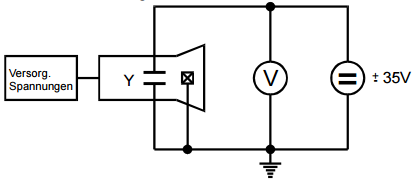
\includegraphics[height=5cm]{picture/Schaltung1}
  \caption{Aufbau zur Messung der Leuchtfleckverschiebung in Abhängigkeit von der Ablenkspannung. \cite[5]{V501}}
  \label{fig:Schaltung1}
\end{figure}

Nun wird der Leuchtfleck, durch ändern der Ablenkspannung $U_\text{d}$ so verschoben, dass dieser auf die neun äquidistanten Linien der y-Achse trifft. Sobald der Leuchtfleck auf einer der Linien ist wird die Ablenkspannung $U_\text{d}$ und die Auslenkung $D$ des Leuchtflecks notiert. \\
Im zweiten Teil des Versuches wird an die y-Ablenkung der Kathodenstrahlröhre ein Sinusgenerator angeschlossen und an die x-Ablenkung ein Sägezahngenerator. Zusätzlich wird an den Sägezahngenerator noch ein Frequenzzähler montiert (siehe Abbildung \eqref{fig:Schaltung2}).

\begin{figure}[H]
  \centering
  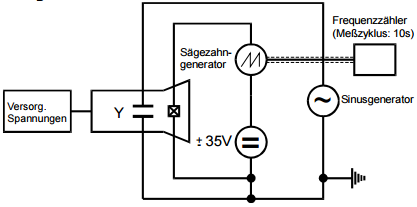
\includegraphics[height=5cm]{picture/Schaltung2}
  \caption{Aufbau für ein Kathodenstrahl-Oszillographen. \cite[5]{V501}}
  \label{fig:Schaltung2}
\end{figure}

Die Frequenz des Sinusgenerators ist bekannt und es wird nun durch Variation der Sägezahnfrequenz versucht stehende Wellen auf den Oszillographen zu erhalten. Die stehenden Wellen tretten bei einem Verhältnis der Sägezahnfrequenz $\nu_\text{sä}$ und der Sinusfrequenz $\nu_\text{si}$ von $n = \frac{1}{2}$, 1, 2 und 3 auf. Für jede stehenden Welle wird die Amplitude (y-Achse) und die Frequenz der Sägezahnspannung aufgeschrieben.

\subsection{Aufbau und Durchführung für das Elektron im B-Feld}
Vor Versuchsbeginn muss mit Hilfe eines Deklinatorium-Inklinatorium die Feldrichtung und der Inklanationswinkel des Erdmagnetfeldes herausgefunden und notiert werden. \\
Der Versuchsaufbau besteht aus einer Helmholtzspule und einer Kathodenstrahlröhre, welche senkrecht zum Magnetfeld der Spule steht. Nun wird der Versuchsaufbau so gedreht, dass die Kathodenstrahlröhre parallel zur horizontal Komponente des Erdmagnetfeldes ausgerichtet ist. Dadurch kann das Erdmagnetfeld keine Kraft auf die Elektronen in der Kathdodenstrahlröhre ausüben. Nun wird der Leuchtfleck mit dem Ablenksystem welches in der Kathodenstrahlröhre verbaut ist auf die unterste Linie des Koordinatensystems gebracht. Danach wird das Magnetfeld der Helmholtzspulen verstärkt, in dem die die Stromstärke erhöht wird. Ähnlich wie im ersten Versuch wird nun die Stromstärke solange erhöht bis der Leuchtfleck eine der neun äquidistanten Linien des Koordinatensystem berührt und es werden die Stromstärke $I$ und die Ablenkung $D$ notiert. \\
Für den zweiten Teil des Versuches wird die Stromstärke der Helmholtzspulen auf null gedreht und die Ablenkspannung der Kathodenstrahlröhre so eingestellt das der Leuchtfleck die mittlere Linie des Koordinatennetzes trifft. Daraufhin wird der Versuchsaufbau un 90 Grad gedreht, sodass der der Leuchtfleck durch das Erdmagnetfeld abgelenkt wird. Nun wird die Stromstärke der Spule solange hochgedreht bis der Leuchtfleck wieder in der mitte des Koordinatennetzes ist. Aus der notierten Stromstärke, kann die Flussdichte $B$ des Erdmagnetfeldes bestimmt werden.  




























asd
